%!TEX TS-program = pdfLaTeX
%!TEX encoding = utf-8
%!TEX spellcheck = en-US

\documentclass[12pt,twoside,openright]{article}

%nœud

%\usepackage{soul}

%\documentclass[a4paper,11pt]{book}
\usepackage[T1]{fontenc}
\usepackage[utf8]{inputenc}
\usepackage[francais]{babel}

\usepackage[usenames,dvipsnames]{color}

\usepackage{lmodern}
%%%%%%%%%%%%%%%%%%%%%%%%%%%%%%%%%%%%%%%%%%%%%%%%%%%%%%%%%
% Source: http://en.wikibooks.org/wiki/LaTeX/Hyperlinks %
%%%%%%%%%%%%%%%%%%%%%%%%%%%%%%%%%%%%%%%%%%%%%%%%%%%%%%%%%
\usepackage{hyperref}
\usepackage{graphicx}
\usepackage{pdfpages}
\usepackage{amsmath}
\usepackage{amssymb}
\usepackage{a4}
\usepackage{indentfirst}
\usepackage{fancyhdr}
\usepackage{varioref}
\usepackage{makeidx}

%\usepackage{biblatex}
\usepackage{mslapa}

\usepackage[normalem]{ulem}



%% Apalike hyphenation %%%
%\let\oldbibitem=\bibitem
%\renewcommand{\bibitem}[2][]{\oldbibitem[#1]{#2}\newline}

%%% Margins %%%
\voffset -2.54cm
\textheight 24cm
\hoffset -1.3in
\evensidemargin 2.5cm
\oddsidemargin 2.5cm
\textwidth 18cm

% Book's title and subtitle
\title{\textbf{A three-party generative model for active foveated vision} }
% Author
\author{\textsc{Emmanuel Daucé}}%\thanks{\url{www.example.com}}}
\date{}
\makeindex

\begin{document}
	
\maketitle


	
\section{Introduction}

In contrast with goal-oriented activity, animal motor activity also relates to the search for sensory clues in order to better understand its sensory environment. This resorts to choosing relevant viewpoints, i.e. selecting body placement and/or sensors orientation in order to capture a sensory signal that should help disambiguate the current scene. It corresponds to selecting views (from a large range of possible views) in order to maximize scene understanding under limited resources constraints. This task is the one considered in this paper (further on called the \emph{sensory scene decoding} task). 

%{\color{magenta} Revue de litterature}

%\paragraph{Multi-view image processing}

Scene decoding through action (or ``active perception'') has attracted strong interest in robotics and artificial vision.  
It mostly refers to the oculo-motor activity, for the movements of the eyes is a salient feature of superior vertebrates vision. The oculo-motor activity is an essential component of man and animal behavior, underlying most of daily displacements, movements, instrumental and social interactions. By moving the gaze with the eyes, the center of sight is constantly and actively moving around during all waking time. 
A salient feature of superior vertebrates visual apparatus is the foveated retina that concentrates  photoreceptors over a small central portion of the visual field \cite{osterberg1935topography}. The scanning of the visual scene is principally done with high-speed targeted eye movements called saccades \cite{yarbus1967eye}, that sequentially capture local chunks of the visual scene. 
Though ubiquitous in biology, object recognition through saccades is seldom considered in artificial vision. 
%The reasons are many, of which the existence of high-performance sensors that provide millions of pixels at low cost.
The opportunity to neglect large parts of the {\color{blue} visual/sensory} should however be considered when the energy is scarce, for the important redundancy present in the {\color{blue} visual/sensory} data allows to envisage energy-efficient visual exploring devices  
using only little portions of the total sensory scene.

%itself, with critical or useful information only present in 

 %Though taking a large part in brain activity, the principles underlying those visually guided movements are still a subject of debate in neurosciences.
%The most documented case of active perception is gaze orientation, primarily studied in both man and animal \cite{yarbus1967eye,robinson1968eye}. A nice review of principal promises of \emph{animate} vision against passive vision  is presented in \cite{ballard1991animate},  in relation with eye-hand coordination in computer vision.
%
%, {\color{magenta} following an approximate exponential decrease of resolution from the center to the periphery [REF?]}. 
 %\footnote{in contrast with animals retina whose actual design relies on a long optimization process under severe resource constraints.}.
%Increasingly powerful computing devices are then assigned to compute in parallel those millions of pixels to perform recognition, consuming resources in a brute-force fashion. 

The example of animal vision thus encourages a more parsimonious approach to computer vision \emph{including the control of the sensory flow}. 
%A salient aspect of animal vision is the use of \emph{active} sensing devices, capable of moving around under some degrees of freedom in order to choose a particular viewpoint. The existence of a set of possible sensor movements calls for the development of specific algorithms that should \emph{solve the viewpoint selection problem}. 
A computer vision program should for instance look back from past experience to see which viewpoint to use to provide the most useful information about a scene. Optimizing the sensor displacements across time may then be a part of computer vision algorithms, in combination with traditional pixel-based operations. 

Changing the viewpoint can be seen as a way to leverage ambiguities present in the current visual field. In \cite{aloimonos1988active}, the authors show that some ill-posed object recognition problems become well-posed as soon as several views on the  same object are considered. 
A more general perspective is developed in \cite{bajcsy1988active}, with a first attempt to interpret active vision in the terms of sequential Bayesian estimation:
\begin{quote}
	\emph{The problem  of Active Sensing can be stated as a problem of controlling strategies 
		applied to the data acquisition process which will depend on the current state 
		of the data interpretation and  the  goal  or the  task of  the  process.}
\end{quote}
thus providing a roadmap for the development of active artificial vision systems.

Selecting 

multi-view image-processing

The active vision literature considers the case of 




further developed in \cite{najemnik2005optimal,butko2010infomax,ahmad2013active,potthast2016active}.



{ different strategies can be adopted to refine the inference accuracy. One way to refine the posterior estimate is to **actively sample** the environment. This is called active inference.} 



\section{Material and methods}

\subsection{Perception-driven control}

\subsubsection{Generative process}
A feedback control framework is composed of an actor and an environment. The actor and the environment interact according to a feedback loop. 
The actor can act on the environment through its effectors, and sense the state of the environment through its sensors. 
The state of the environment as well as the state of the agent can change over time. The state of the environment is described by a state vector $\boldsymbol{z} \in \mathcal{Z}$.
In a Markovian framework, the state $\boldsymbol{z}$ in which the physical system is found at present depend both on its previous state (say $\boldsymbol{z}_0$) and on a preceding motor command $\boldsymbol{u}$ 
The transition from $\boldsymbol{z}_0$ to $\boldsymbol{z}$ is reflected in a \emph{transition function} that embodies the deterministic and non-deterministic effects of the command $\boldsymbol{u}$ in a conditional probability distribution:  
\begin{align}
\boldsymbol{z} \sim \text{Pr}(Z|\boldsymbol{u},\boldsymbol{z}_0) \label{eq:process}
\end{align}
implemented with a probability density function 
$p_\text{\sc trans}(\boldsymbol{z}|\boldsymbol{u},\boldsymbol{z}_0)$.


The signal $\boldsymbol{x}$ that is measured on the sensors is called the \emph{sensory field}. It is interpreted as a measure made by the sensors, that is causally related to the current state $\boldsymbol{z}$ and motor command $\boldsymbol{u}$. Once again the deterministic and non-deterministic effects are reflected in a conditional probability distribution:
\begin{align}
\boldsymbol{x} \sim \text{Pr}(X|\boldsymbol{z},\boldsymbol{u})\label{eq:measure}
\end{align}
implemented with a probability density function 
$p_\text{\sc meas}(\boldsymbol{x}|\boldsymbol{z},\boldsymbol{u})$.
The combination of  (\ref{eq:process}) and (\ref{eq:measure}) is said a \emph{generative process} that is the cause of the sensory field. 

%{\color{magenta} probabilistic framework : the changes that take place in the physical world described by  = model.}
%Given an initial state $\boldsymbol{z}_0$, the next state $\boldsymbol{z}$ rests on the conditional distribution   and the 

\subsubsection{Inference}

When both the transition and the measure models are known, it is possible to \emph{infer} the latent state of the physical system $\boldsymbol{z}$ from the sensory field $\boldsymbol{x}$, the previous state $\boldsymbol{z}_0$ and the motor command $\boldsymbol{u}$ using Bayes rule:
\begin{align}
\text{Pr}(Z|X,\boldsymbol{u},\boldsymbol{z}_0) = \frac{\text{Pr}(X,Z|\boldsymbol{u},\boldsymbol{z}_0)}{\text{Pr}(X|\boldsymbol{u},\boldsymbol{z}_0)} %\nonumber 
= \frac{\text{Pr}(X|Z,\boldsymbol{u}) \text{Pr}(Z|\boldsymbol{u},\boldsymbol{z}_0)}
{\text{Pr}(X|\boldsymbol{u},\boldsymbol{z}_0)}\label{eq:post-Pr}
%&= \frac{\text{Pr}(X|Z,\boldsymbol{u}) \text{Pr}(Z|\boldsymbol{u},\boldsymbol{z}_0)}{\sum_{\boldsymbol{z}'}\text{Pr}(X|\boldsymbol{z}',\boldsymbol{u}) \text{Pr}(\boldsymbol{z}'|\boldsymbol{u},\boldsymbol{z}_0)}\label{eq:post}
\end{align}
where $P(Z|X,\boldsymbol{u},\boldsymbol{z}_0)$ is the \emph{posterior} probability (a distribution over the latent states) whose order 2 moment informs on the estimation accuracy : the narrower the distribution, the more accurate the latent state prediction. 
The inference of the latent state through model inversion is called \emph{filtering} for it serves to refine the actual state estimate from past observations when the measure process is corrupted by noise \cite{Kalman1960}.
It may be implemented with a probability density function:
\begin{align}
q_\text{\sc post}(\boldsymbol{z}|\boldsymbol{x},\boldsymbol{u}, \boldsymbol{z}_0) 
= \frac{p_\text{\sc meas}(\boldsymbol{x}|\boldsymbol{z},\boldsymbol{u}) p_\text{\sc trans}(\boldsymbol{z}|\boldsymbol{u},\boldsymbol{z}_0)}
{\sum_{\boldsymbol{z}'}p_\text{\sc meas}(\boldsymbol{x}|\boldsymbol{z}',\boldsymbol{u}) p_\text{\sc trans}(\boldsymbol{z}'|\boldsymbol{u},\boldsymbol{z}_0)}\label{eq:post-pdf}
\end{align}

\subsubsection{One scene, many views}
An important special case is when the motor command only relates to the \emph{orientation of a sensor}. The motor command $\boldsymbol{u}$ then corresponds to the desired end-orientation of the sensor here considered as a setpoint on the actuators space, either expressed in actuators or endpoint coordinates (with hardware-implemented detailed effector response function).  
Under that perspective, the effector acts on the sensors position and orientation so as to achieve a certain perspective (or view) over the external scene. The motor control $\boldsymbol{u}$ is now called a \emph{viewpoint} and most importantly \emph{is not expected to affect on the latent state $\boldsymbol{z}$}, i.e.
\begin{align}
\boldsymbol{z} \sim \text{Pr}(Z|\boldsymbol{z}_0)
\end{align} 
so that $\boldsymbol{z}$ should depend only on the external dynamics (the external ``uncontrolled'' process).


Under a scene decoding  task, where the motor command $\boldsymbol{u}$ refers to the orientation of a sensor, it is rather common to consider the environment as ``static'' \cite{butko2010infomax}. This means, in short, that:
$$\text{Pr}(Z|\boldsymbol{z}_0) = \delta(Z, \boldsymbol{z}_0)$$ 
with $\delta$ the Knonecker symbol. 
The latent variable $\boldsymbol{z}$ is thus expected to capture all relevant information about the current scene, while remaining invariant throughout the decoding process. In a model-based approach, it may specify the state of the physical environment. In a model-free view, it should be expressive enough to restore information about the environment.  

Each different viewpoint $\boldsymbol{u}$ can be seen as a different sensory fields over the same underlying sensory scene, and $\boldsymbol{x}$ (the view) is the realization of a generative model parametrized by $\boldsymbol{u}$ and $\boldsymbol{z}$. This generative model is written:
$$p(X, Z, U) = p_\text{\sc meas}(X| Z, U)p_\text{\sc prior}(Z, U)$$
It can further on be simplified by considering that the measure captures all the relevant dependencies, i.e. that $X$ is conditionally dependent on the $(U,Z)$ couple, but independent from $U$ alone and independent from $Z$ alone, while $U$ and $Z$ are also mutually independent, i.e.:
$$p(X, Z, U) = p_\text{\sc meas}(X| Z, U)p_\text{\sc prior}(Z) p_\text{\sc prior}(U)$$


The dependencies between the three variables can moreover be symetrically decomposed in the form of three conditional models, i.e. :
\begin{align}
	p(X, Z, U) &= p(X| Z, U) p(Z)p(U)\nonumber\\ 
	&= p(Z| X, U)p(X) p(U)\nonumber\\
	&= p(U|X, Z)p(X) p(Z)\nonumber
\end{align}
comprising a \emph{forward model} $p(X|\boldsymbol{z}, \boldsymbol{u})$ 
conditioned on both $\boldsymbol{z}$ and $\boldsymbol{u}$,  an \emph{inverse model} $p(Z|\boldsymbol{x}, \boldsymbol{u})$  conditioned on both on  $\boldsymbol{x}$ and $\boldsymbol{u}$ and an ``\emph{inverse controller}'' $p(U|\boldsymbol{x}, \boldsymbol{z})$ conditioned on both on  $\boldsymbol{x}$ and $\boldsymbol{z}$. This boils down to implementing three variants of a two \emph{degrees of freedom} generative model. 

\subsubsection{Scene encoding and scene decoding}

\paragraph{Scene encoding}
The \emph{variational encoding} perspective \cite{hinton1994autoencoders} was originally developed 
to train unsupervised autoencoder neural networks. The general idea is that an efficient code 
is a code that is both compact and accurate at restoring the data. 
If $\boldsymbol{x}$ is the original data, the corresponding code $\boldsymbol{z}$ is generated by a distribution $q$, i.e. $\boldsymbol{z} \sim q(Z)$. This distribution is called the \emph{encoder}. Then, the reconstruction is made possible with a second conditional probability over the codes, i.e. $p(X|\boldsymbol{z})$, that is called the \emph{decoder}. If $\boldsymbol{z}$ is the current code, the reconstructed data is $\tilde{\boldsymbol{x}} \sim p(X|\boldsymbol{z})$. 
 
In short, the efficacy of a code is estimated by an information-theoretic quantity, the ``reconstruction cost'' that is defined for every $\boldsymbol{x}$ knowing $p$ and $q$:
\begin{align}
F(\boldsymbol{x}) &= - \sum_{\boldsymbol{z} \in \mathcal{Z}} q(\boldsymbol{z}) \log (p(\boldsymbol{x}|\boldsymbol{z})p(\boldsymbol{z})) - H(q)\nonumber\\
&= \mathbb{E}_{z\sim q} \left[-\log (p(\boldsymbol{x}|\boldsymbol{z})p(\boldsymbol{z}))\right] - H(q)
\label{eq:FEP-energy}
\end{align}
with $\mathcal{Z}$ an arbitrary encoding space, $q$ an arbitrary distribution over the codes, $H(q) = -\sum_z q(\boldsymbol{z}) \log q(\boldsymbol{z})$ the entropy of $q$, $p(X|Z)$ the decoder and $p(Z)$ a prior distribution over the codes.
The densities $p$ and $q$ are called ``variational'' for they can be optimized according to the data \cite{hinton2006fast,kingma2013auto}.  
$F$ is also called the variational free energy for it is mathematically analog to the Helmhotz Free Energy.
It can then be shown, with some reordering, that:
\begin{align}
F(\boldsymbol{x}) 
&= - \log p(\boldsymbol{x}) + \text{KL}(q(Z)||p(Z|\boldsymbol{x}))
\label{eq:FEP}
\end{align}
so that an optimal code $q(Z)\simeq p(Z|\boldsymbol{x})$ can be optimized through a stochastic gradient descent over $p$ and $q$ according to $\nabla_{p,q} F(\boldsymbol{x}) $	 --~see \cite{kingma2013auto}~-- so that the reconstruction cost should meet the ``description length'' of the data, i.e. its estimated (natural) Shannon Information under the model $p$:
$$h(\boldsymbol{x}) \simeq -\log p(\boldsymbol{x}) %\simeq - \log \sum_{\boldsymbol{z} \in \mathcal{Z}} p(\boldsymbol{x},\boldsymbol{z})  
$$
that is a quantity representing how unlikely $\boldsymbol{x}$ is regarding the data model $p$. Minimizing $F$ according to $p$ and $q$ thus means minimizing the ``surprise'' caused by observing $\boldsymbol{x}$ \cite{friston2010free}.
 
 
%, that is composed of two terms, namely the reconstruction accuracy $- \mathbb{E}_{\boldsymbol{z}\sim q} \log p(\boldsymbol{x}|\boldsymbol{z})$ and the Kullback-Leibler divergence $\text{KL}(q||\rho)$ between the current code $q$ and a  
%An efficient encoder is thus obtained by minimizing $F$ by gradient descent over $p$ and $q$, given a dataset $\{\boldsymbol{x}_1, ..., \boldsymbol{x}_n\}$ \cite{Kingma...}.  
 
If we now turn back to the viewpoint selection setup, an additional factor $\boldsymbol{u}$ (the viewpoint) comes into the play. The data $\boldsymbol{x}$ that is actually read is now conditioned on  $\boldsymbol{u}$, so that:
\begin{align}
F(\boldsymbol{x}|\boldsymbol{u}) 
&= \mathbb{E}_{z\sim q} \left[-\log (p(\boldsymbol{x}|\boldsymbol{z},\boldsymbol{u})p(\boldsymbol{z}))\right] - H(q)\\
&= \mathbb{E}_{z\sim q} \left[-\log (p(\boldsymbol{x}|\boldsymbol{z},\boldsymbol{u}))\right] +\text{KL}(q(Z)||p(Z))
\label{eq:FEP-prior-u}\\
&= - \log p(\boldsymbol{x}|\boldsymbol{u}) + \text{KL}(q(Z)||p(Z|\boldsymbol{x}, \boldsymbol{u}))
\label{eq:FEP-posterior-u}\end{align}
with each viewpoint $\boldsymbol{u}$ providing a distinct optimization problem. 
 
\paragraph{Scene decoding}
The structure of the problem (many views on the same scene) implies that the different possible measures should share a common information corresponding to the actual (covered) sensory scene. The sharing of information between two sensory fields can be quantified by their \emph{mutual information} (or ``Information gain'' --~see \cite{tishby2011information}~--):
\begin{align}
I((X| \boldsymbol{u}); (X'| \boldsymbol{u}')) &\simeq \mathbb{E}_{X,X'} \left[-\log p(X| \boldsymbol{u}) + \log p(X'| \boldsymbol{u}', X, \boldsymbol{u})\right] \nonumber\\
&\simeq \mathbb{E}_{X,X'} \left[F(X|\boldsymbol{u}) - F(X'|\boldsymbol{u}', X, \boldsymbol{u})\right] 
\end{align}
with $F(\boldsymbol{x}'|\boldsymbol{u}', \boldsymbol{x}, \boldsymbol{u})$ approaching  $-\log p(\boldsymbol{x}'| \boldsymbol{u}', \boldsymbol{x}, \boldsymbol{u})$, which is the approximate natural Shannon Information provided by seeing $\boldsymbol{x}'$ at $\boldsymbol{u}'$ after seeing $\boldsymbol{x}$ at $\boldsymbol{u}$. The quantity $-\log p(\boldsymbol{x}'| \boldsymbol{u}', \boldsymbol{x}, \boldsymbol{u})$ can be expressed through a ``chain rule'': 
\begin{align}
-\log p(\boldsymbol{x}'| \boldsymbol{u}', \boldsymbol{x}, \boldsymbol{u}) 
&\leq - \sum_z q(z) \log p(\boldsymbol{x}'| \boldsymbol{u}', \boldsymbol{z}) \frac{p(\boldsymbol{z} |\boldsymbol{x}, \boldsymbol{u})} {q(z)}  \nonumber\\
&\stackrel{q(z) = p(\boldsymbol{z} |\boldsymbol{x}, \boldsymbol{u})}{\simeq} 
- \sum_z p(\boldsymbol{z} |\boldsymbol{x}, \boldsymbol{u}) \log p(\boldsymbol{x}'| \boldsymbol{u}', \boldsymbol{z})  \nonumber\\
&= \mathbb{E}_{\boldsymbol{z} \sim p(Z |\boldsymbol{x}, \boldsymbol{u})} \left[-\log p(\boldsymbol{x}'| \boldsymbol{u}', \boldsymbol{z})\right] 
\end{align}
So that:
\begin{align}
F(\boldsymbol{x}'|\boldsymbol{u}', \boldsymbol{x}, \boldsymbol{u}) 
&\triangleq \mathbb{E}_{\boldsymbol{z} \sim q} \left[-\log p(\boldsymbol{x}'| \boldsymbol{u}', \boldsymbol{z})\right] + \text{KL}(q(Z)||p(Z|\boldsymbol{x},\boldsymbol{u}))
\label{eq:FEP-uxu}
\end{align}
which is a special case of the POMDP\footnote{Partially Observed Markov Decision Processes.} variational Free Energy formulation proposed in \cite{friston2015active}.

If we look in detail, the posterior $p(Z|\boldsymbol{x},\boldsymbol{u})$ plays the same role as the prior in eq. (\ref{eq:FEP-prior-u}). This reflects the chaining of the posterior to the role of the prior in the next estimation step, a typical property of sequential Bayesian inference {\color{magenta}(ref??)}.
Such chaining can be generalized to many observations: $(\boldsymbol{x},\boldsymbol{u}), (\boldsymbol{x}',\boldsymbol{u}'), ... , (\boldsymbol{x}^{(n)},\boldsymbol{u}^{(n)})$ issuing a final scene decoding $q^{(n)}(Z)$:
$$ q^{(n)}(Z) \propto p(Z|\boldsymbol{x},\boldsymbol{u}) p(Z|\boldsymbol{x}',\boldsymbol{u}') ... p(Z|\boldsymbol{x}^{(n)},\boldsymbol{u}^{(n)}) $$\\
It is noteworthy that the $\boldsymbol{u}$'s and $\boldsymbol{x}$'s do not need to be stored in the process. At step $n$, only $q^{(n-1)}$ (the current ``belief'') needs to be memorized to estimate $q^{(n)}$, i.e. 
$$ q^{(n)}(Z) \propto p(Z|\boldsymbol{x},\boldsymbol{u}) q^{(n-1)}(Z) $$

Finally, from the encoding point of view, the $n^\text{th}$ reconstruction cost $F^{(n)}(\boldsymbol{x}^{(n)}|\boldsymbol{u}^{(n)}, ..., \boldsymbol{x}, \boldsymbol{u})$ also obeys to the chain rule, i.e. is estimated from $q^{(n-1)}$, $\boldsymbol{u}^{(n)}$ and $\boldsymbol{x}^{(n)}$ only:
\begin{align}
F(\boldsymbol{x}^{(n)}|\boldsymbol{u}^{(n)}, ...,  \boldsymbol{x}, \boldsymbol{u}) 
&= \mathbb{E}_{\boldsymbol{z} \sim q^{(n)}} \left[-\log p(\boldsymbol{x}^{(n)}| \boldsymbol{u}^{(n)}, \boldsymbol{z})\right] + \text{KL}(q^{(n)}(Z)||q^{(n-1)}(Z))
\label{eq:FEP-uxun}
\end{align}
%The posterior of a prior step has been passed to the next estimation step and now plays the role of the prior.  This shows that a single distribution $q_\text{\sc post}(Z_{t-1})$ needs to be conserved in memory to calculate the next estimate $q_\text{\sc post}(Z_t)$, i.e.:
with $q^{(n)}(Z)$ the shared (or cumulative) encoding according to the past and current observations, providing a \emph{forward} variational encoding scheme (see also \cite{fraccaro2016sequential} for a backward variational encoding scheme). 


\subsection{Action selection and scene decoding optimization}
Consider now an agent whose objective is to precisely estimate its environment state $\boldsymbol{z}$ from its sensory field and a generative model $G = (p_\text{\sc trans}; p_\text{\sc meas};p_\text{\sc prior})$.
Depending on $\boldsymbol{u}$ (current viewpoint), a different $\boldsymbol{x}$ is observed at the sensors. So, each different command $\boldsymbol{u}$ provokes a different observation, and thus a different 
estimation of the latent state. It is thus worth to question what is the optimal choice for $\boldsymbol{u}$ in order to maximize the accuracy of the posterior estimate?

Considering that the effect of the action $\boldsymbol{u}$ on the next observation $\boldsymbol{x}$ is not known in advance, different strategies can be adopted to choose $\boldsymbol{u}$ in a way that is expected to maximize the accuracy of the environment's state estimation. This approach to inference is called \emph{active sampling}, for the choice of $\boldsymbol{u}$ determines the sensory sample $\boldsymbol{x}$ that is observed, conditioning the final posterior estimate.

A baseline sampling strategy is to choose $\boldsymbol{u}$ at random and condition the posterior  estimate on this random action. 
More elaborate strategies consider the past state $\boldsymbol{z}_0$ to choose the most promising action $\boldsymbol{u}$ (regarding next posterior accuracy). The problem turns out to design  a \emph{controller} $C$. A controller is a function that, given a context $\boldsymbol{z}_0$, sets up an action $\boldsymbol{u} = C(\boldsymbol{z}_0)$. The role of that controller is not to achieve a certain task, but only to render the estimation of the (future) outer state more accurate. The controller is said \emph{perception-driven}. 

The design of such a controller is not straightforward. On contrary to classical control, there is not definite setpoint $\boldsymbol{z}^*$ to which the controller is supposed to drive the external process (through model inversion for instance). By design, the actual outer state $\boldsymbol{z}$ is not visible as such and can not be compared to the inferred posterior. A general strategy is thus to establish a \emph{objective function} $f$ (resp. a loss $\ell$) that conveys a quantitative estimation of the action's contribution to the inference accuracy (resp. imprecision). Once the objective function established, a simple control strategy is to choose the action that maximizes the objective (resp. minimizes the loss), i.e.:
\begin{align}
\hat{\boldsymbol{u}} = \underset{\boldsymbol{u}\in\mathcal{U}}{\text{argmax}}  f(\boldsymbol{z}_0, \boldsymbol{u})
\end{align}

Many such objective functions are proposed in the literature. They are generally referred as an \emph{intrinsic} motivation by contrast with the \emph{extrinsic} motivation that relates to the classical rewards in reinforcement learning \cite{sutton1998reinforcement}. Several intrinsic reward candidates are developed and commented in the following sections.

{\color{magenta} la stratégie générale consiste à définir une fonction objectif permettant d'estimer la qualité du contrôle effectué selon un critère de précision de l'estimation d'état. Cadre du RL? Le problème des etats explicites (non markovien) et le principe de l'état caché.}

{\color{blue} 
	\begin{itemize}
		\item error-based objective
		\item accuracy-based
		\item information-based (Infomax, information gain)
		\item curious / diversity based  (Schmidhuber, Open AI)
	\end{itemize}
	
	
	The perception-driven control objective is defined for any kind of effector and any kind of motor control.} 

\subsection{The POMDP framework}

The presented action selection framework can be repeated over time to form a sequential state estimation process. 
The initial viewpoint at time $t=0$ is noted $\boldsymbol{u}_0$, and the subsequent viewpoints  are noted $\boldsymbol{u}_1, \boldsymbol{u}_2, ...$ with $\boldsymbol{u}_{0:T-1}$ describing a sequence of $T$ viewpoints from $t=0$ to $t=T-1$. % (with a corresponding random variable $U_{0:T}$ under a probabilistic framework).

In a state estimation process, the state of the environment at time 0, i.e. $\boldsymbol{z}_0$, is not directly visible. This latent state can only be disclosed step by step through sensing the world from different viewpoints. Initially, in the absence of a measure, it is described by a prior distribution over the initial states noted $p_\text{\sc prior}(\boldsymbol{z}_0)$. At the end of a trial, the final state estimate is best described by a conditional probability over the actual sequence of controls $\boldsymbol{u}_{0:T-1}$ and the corresponding observations $\boldsymbol{x}_{1:T}$, i.e. :
$$\text{Pr}(Z_{0:T}|\boldsymbol{u}_{0:T-1}, \boldsymbol{x}_{1:T})$$

\begin{figure}[t!]
	\centerline{
		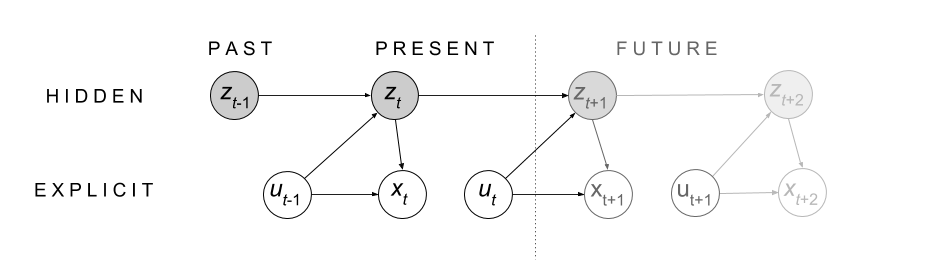
\includegraphics[width = \linewidth]{img/ICLR-graphical-v2.png} 
	}
	\caption{Graphical generative model (see text)}\label{fig:pomdp}
\end{figure}


To implement such an estimation process, the Partially-Observed Markov Decision Process (POMDP) framework is generally considered. It tells, in short, that the current hidden state $\boldsymbol{z}_t$ is only conditionally dependent on the previous hidden state $\boldsymbol{z}_{t-1}$, the previous control $\boldsymbol{u}_{t-1}$ and the current observation $\boldsymbol{x}_t$ (see figure \ref{fig:pomdp}). 
The POMDP framework has been extensively developed in the context of active vision \cite{butko2010infomax,ahmad2013active,potthast2016active}.
Given a generative model $G = (p_\text{\sc prior}; p_\text{\sc trans}; p_\text{\sc meas})$, the forward estimate for $\boldsymbol{z}_{0:t}$ at time $t$ is provided by a sequential recursive update: 
$$q_\text{\sc post}(\boldsymbol{z}_{0:t}|\boldsymbol{x}_{1:t},\boldsymbol{u}_{0:t-1}) 
= \frac{p_\text{\sc meas}(\boldsymbol{x}_t|\boldsymbol{z}_t,\boldsymbol{u}_{t-1}) p_\text{\sc trans}(\boldsymbol{z}_t|\boldsymbol{u}_{t-1},\boldsymbol{z}_{t-1})}
{\sum_{\boldsymbol{z}_t'}p_\text{\sc meas}(\boldsymbol{x}_t|\boldsymbol{z}_t',\boldsymbol{u}_{t-1}) p_\text{\sc trans}(\boldsymbol{z}_t'|\boldsymbol{u}_{t-1},\boldsymbol{z}_{t-1})} \times q_\text{\sc post}(\boldsymbol{z}_{0:t-1}|\boldsymbol{x}_{1:t-1},\boldsymbol{u}_{0:t-2}, \boldsymbol{z}_{0:t-2}) \label{eq:post-pompd}$$
with $q_\text{\sc post}(\boldsymbol{z}_0) = p_\text{\sc prior}(\boldsymbol{z}_0)$.

To simplify writing, the local posterior estimate is noted :
$$ \Delta q_\text{\sc post}(\boldsymbol{z}_t|\boldsymbol{x}_t,\boldsymbol{u}_{t-1}, \boldsymbol{z}_{t-1}) 
\triangleq \frac{p_\text{\sc meas}(\boldsymbol{x}_t|\boldsymbol{z}_t,\boldsymbol{u}_{t-1}) p_\text{\sc trans}(\boldsymbol{z}_t|\boldsymbol{u}_{t-1},\boldsymbol{z}_{t-1})}
{\sum_{\boldsymbol{z}_t'}p_\text{\sc meas}(\boldsymbol{x}_t|\boldsymbol{z}_t',\boldsymbol{u}_{t-1}) p_\text{\sc trans}(\boldsymbol{z}_t'|\boldsymbol{u}_{t-1},\boldsymbol{z}_{t-1})}
$$

so that :

\begin{align}
q_\text{\sc post}(\boldsymbol{z}_{0:t}|\boldsymbol{x}_{1:t},\boldsymbol{u}_{0:t-1}) 
%&= \Delta q_\text{\sc post}(\boldsymbol{z}_t|\boldsymbol{x}_t,\boldsymbol{u}_{t-1}, \boldsymbol{z}_{t-1})  
%\times q_\text{\sc post}(\boldsymbol{z}_{t-1}|\boldsymbol{x}_{1:t-1},\boldsymbol{u}_{0:t-2}, \boldsymbol{z}_{0:t-2})\nonumber\\
&= \Delta q_\text{\sc post}(\boldsymbol{z}_t|\boldsymbol{x}_t,\boldsymbol{u}_{t-1}, \boldsymbol{z}_{t-1})  
\times ... \times \Delta q_\text{\sc post}(\boldsymbol{z}_1|\boldsymbol{x}_1,\boldsymbol{u}_0, \boldsymbol{z}_0)  \times  p_\text{\sc prior}(\boldsymbol{z}_0) \nonumber
\end{align}

The forward probabilistic estimate of a path $\boldsymbol{z}_{0:t}$ is thus the product of $t$ co-dependent posterior estimates (for $\boldsymbol{z}_t$ is conditionally dependent on $\boldsymbol{z}_{t-1}$ etc.), where the co-dependence implements a one-step \emph{memory} of the past state estimates. In practice, in a forward scheme, only a single distribution $q_\text{\sc post}(Z_{t-1})$ needs to be conserved in memory to calculate the next estimate $q_\text{\sc post}(Z_t)$, i.e.:
$$q_\text{\sc post}(Z_t|\boldsymbol{x}_t,\boldsymbol{u}_{t-1}, Z_{t-1}) = 
\Delta q_\text{\sc post}(Z_t|\boldsymbol{x}_t,\boldsymbol{u}_{t-1}, Z_{t-1}) 
\times q_\text{\sc post}(Z_{t-1}|\boldsymbol{x}_{t-1},\boldsymbol{u}_{t-2}, Z_{t-2})$$
where $q_\text{\sc post}(Z_{t-1}|\boldsymbol{x}_{t-1},\boldsymbol{u}_{t-2}, Z_{t-2})$ is the only needed information to estimate $Z_t$. It is thus the formal equivalent of a prior in a single step Bayesian inference.
%The corresponding numerical scheme generally relies on a logarithm transform:
%\begin{align}
%\log q_\text{\sc post}(\boldsymbol{z}_{0:t}|\boldsymbol{x}_{1:t},\boldsymbol{u}_{0:t-1}) 
%&= \log \Delta q_\text{\sc post}(\boldsymbol{z}_t|\boldsymbol{x}_t,\boldsymbol{u}_{t-1}, \boldsymbol{z}_{t-1})  
%+ ... + \log \Delta q_\text{\sc post}(\boldsymbol{z}_1|\boldsymbol{x}_1,\boldsymbol{u}_0, \boldsymbol{z}_0)  +  \log p_\text{\sc prior}(\boldsymbol{z}_0) \nonumber
%\end{align}

\subsection{Action selection under the efficient coding perspective}


\subsection{Action selection : the Infomax perspective}

The local information gain is defined as :


\subsection{Action selection : the efficient coding perspective}

\section{Results}

\section{Discussion}

\bibliographystyle{apalike}
\bibliography{biblio}

\end{document}